\documentclass[conference]{IEEEtran}
% \usepackage{cite}
\usepackage{amsmath,amssymb,amsthm,enumitem}
\usepackage{graphicx}
\usepackage{textcomp}
\usepackage{xcolor}
\usepackage{url}
\usepackage{cite}
% Custom theorem environment for a professional look
\newtheorem{theorem}{Theorem}
\newtheorem{lemma}{Lemma}

\def\BibTeX{{\rm B\kern-.05em{\sc i\kern-.025em b}\kern-.08em
    T\kern-.1667em\lower.7ex\hbox{E}\kern-.125emX}}
\begin{document}

\title{Information Flow in Deep Neural Networks Under Distributional Shifts}

\author{
\IEEEauthorblockN{Mohammad Mohammadianbisheh}
\IEEEauthorblockA{\textit{Sharif University of Technology}}
\and
\IEEEauthorblockN{Mohammadamin Kiani}
\IEEEauthorblockA{\textit{Sharif University of Technology}}
\and
\IEEEauthorblockN{Diba Hadi}
\IEEEauthorblockA{\textit{Sharif University of Technology}}
}

\maketitle

\begin{abstract}
Understanding the internal mechanisms of deep neural networks (DNNs) remains a critical challenge. Information-theoretic measures, such as mutual information, offer a principled way to analyze what DNNs learn. This report builds upon the work of Goldfeld et al.\cite{goldfeld2019estimating} , who developed a rigorous framework for estimating the mutual information between the input and hidden layer representations in noisy DNNs. We first review their Sample Propagation (SP) estimator and its theoretical guarantees, highlighting the connection between information compression and the geometric clustering of representations. Our primary contribution is to extend this analysis by investigating the robustness of the information estimator to shifts in the input data distribution. We derive novel theoretical bounds on the estimator's deviation when the input distribution is perturbed, measured by Total Variation (TV) and Kullback-Leibler (KL) divergence. We supplement our theoretical results with experiments on the SZT and MNIST datasets, demonstrating how information estimates in different layers evolve under these distributional shifts throughout training. Finally, we propose future research directions, including the exploration of Wasserstein distance-based bounds and the application of Distributionally Robust Optimization (DRO) to enhance the stability of information flow.
\end{abstract}


\section{Introduction}

Deep Neural Networks (DNNs) have achieved state-of-the-art performance on a wide array of tasks, yet they are often treated as "black boxes." A fundamental goal of deep learning theory is to understand the principles governing how these networks learn effective representations of data. Information theory provides a powerful lens for this purpose. The Information Bottleneck (IB) principle \cite{shwartz2017opening}, for instance, posits that an optimal representation should compress the input as much as possible while retaining the maximum information about the target variable. This suggests that DNN training involves two distinct phases: an initial fitting phase where the mutual information between hidden layers and the target increases, followed by a compression phase where information about the input is discarded \cite{tishby2015deep}.

Measuring the mutual information $I(X;T)$ between the input $X$ and a hidden layer representation $T$ is notoriously difficult, especially in deterministic networks where it is often ill-defined or vacuous \cite{kolchinsky2019caveats}. To address this, Goldfeld et al. \cite{goldfeld2019estimating} proposed a framework for studying information flow in stochastic DNNs. They introduced additive Gaussian noise to each hidden layer, making the mutual information well-defined and dependent on network parameters. They developed a provably accurate Sample Propagation (SP) estimator to track $I(X;T)$ and provided theoretical bounds on its performance.

A key insight from their work is that the observed compression of $I(X;T)$ is driven by the geometric clustering of hidden representations of inputs from the same class. As training progresses, these representations become less distinguishable, leading to a reduction in mutual information.

While this framework provides a tool for analysis, the robustness of such information-theoretic measures to changes in the data distribution is not well understood. In real-world applications, models often encounter data that differs from the training distribution. Our work extends the analysis of Goldfeld et al. \cite{goldfeld2019estimating} by formally studying the stability of the information estimator under distributional shifts. Specifically, we ask: if the input distribution $P_X$ is perturbed to a nearby distribution $P_{X'}$, how much does the estimated information change?

We derive novel theoretical bounds on the deviation of the information estimator under perturbations measured by Total Variation (TV) and Kullback-Leibler (KL) divergence. We then empirically validate our findings by tracking the information flow in various layers of DNNs trained on the SZT and MNIST datasets while applying controlled perturbations to the input data.

\section{Estimating Information Flow in Deep Neural Networks}

\subsection{A Rigorous Framework: Noisy DNNs}
In a standard deterministic DNN, a hidden representation $T$ is a deterministic function of the input $X$. For continuous inputs and typical nonlinearities, the true mutual information $I(X;T)$ is infinite. To overcome this, Goldfeld et al. \cite{goldfeld2019estimating} propose a noisy DNN model where i.i.d. Gaussian noise is added to the output of each hidden layer. The $l$-th hidden layer is described by:
\begin{equation}
T_l = f_l(T_{l-1}) + Z_l, \quad Z_l \sim \mathcal{N}(0, \beta^2 I)
\label{eq:noisy_layer}
\end{equation}
This stochastic mapping ensures that $I(X;T_l)$ is finite and sensitive to the network's weights.

\subsection{The Sample Propagation (SP) Estimator}
The mutual information is defined by the difference in differential entropies:
\begin{equation}
I(X; T_l) = h(T_l) - \mathbb{E}_{x \sim P_X}[h(T_l | X=x)]
\end{equation}
Directly computing these entropies is intractable. The SP estimator works by approximating the true data distributions with empirical distributions from samples. Given a dataset $\mathcal{X}$, the estimator is given by:
\begin{equation}
\hat{I}_{SP} = h(\hat{P}_{S_l} * \phi_\beta) - \frac{1}{n} \sum_{x \in \mathcal{X}} h(\hat{P}_{S_l|x} * \phi_\beta)
\end{equation}
where $S_l = f_l(T_{l-1})$ is the pre-noise "signal" and $\phi_\beta$ is the PDF of the Gaussian noise.

\subsection{Theoretical Guarantees of the SP Estimator}
Goldfeld et al. \cite{goldfeld2019estimating} provide several guarantees for the SP estimator. They show that it achieves the optimal parametric rate of convergence, with an absolute-error risk bounded as:
\begin{equation}
\sup_{P_X} \mathbb{E}|I(X; T_l) - \hat{I}_{SP}| \le 2\Delta_{\beta,d_l}(n) + \frac{d_l \log(1 + 1/\beta^2)}{4\sqrt{n}}
\label{eq:goldfeld_bound}
\end{equation}
where $\Delta_{\beta,d_l}(n)$ is the risk for a single entropy term. A key finding is that information compression is linked to geometric clustering, as illustrated in Fig. \ref{fig:info_evolution}.

\begin{figure}[!t]
\centering
% ====================================================================
% ====> REPLACE 'figure1_placeholder.png' with your actual figure file.
% ====================================================================
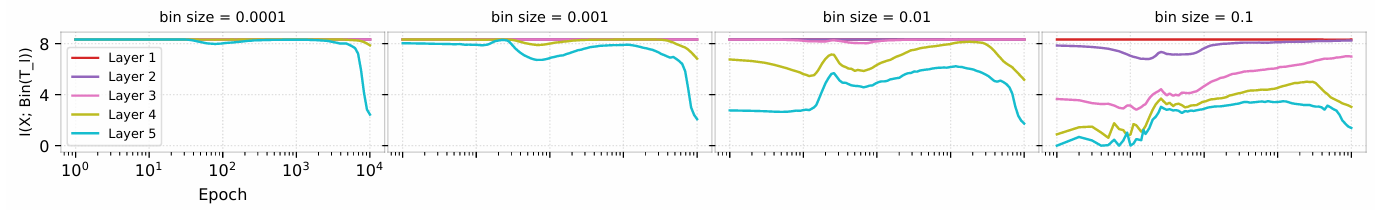
\includegraphics[width=3.4in, height=0.8in]{ITSL/FromPaper.png}
\caption{Evolution of $I(X; T_l)$ for layers during training (adapted from \cite{goldfeld2019estimating}).}
\label{fig:info_evolution}
\end{figure}

\subsection{Estimation Challenges: Sample Complexity}
A core challenge highlighted in \cite{goldfeld2019estimating} is the sample complexity required for accurate estimation. For a hidden layer of dimension $d$, the number of samples $n^*$ needed to achieve a target error $\eta$ has a lower bound that is exponential in $d$:
\begin{equation}
n^*(\eta, \beta, d) \ge \Omega \left( \frac{2^{\gamma(\beta)d}}{d\eta} \right)
\end{equation}
This exponential dependence, often called the "curse of dimensionality," means that accurately estimating mutual information is computationally prohibitive for very wide neural network layers. This motivates the study of how these estimates behave under perturbations, as perfect estimation is often infeasible.

\section{Robustness of Information Estimation}

To derive our robustness bounds, we make a simplifying hypothesis about the output space of the hidden layers. We assume the continuous output of a single neuron can be discretized into $K$ distinct states or bins. This approach is well-justified for networks using bounded activation functions (where $\|f_l\|_{\infty} \le 1$), such as Tanh, as the bounded output space can be approximated with arbitrary precision by increasing $K$. For a layer $l$ containing $d_l$ neurons, the total number of discrete output states for the entire layer representation, $N_l$, becomes $N_l = K^{d_l}$. This allows us to formulate explicit, dimension-aware bounds.

\subsection{Bounding Deviation under TV Shift}
\begin{theorem}
Let $\hat{I}_{SP}$ be the estimator built using n samples from $P_X$. If the data distribution shifts to $P_{X'}$, such that $TV(P_X, P_{X'}) \le \epsilon$, and we assume a discretization of each neuron into $K$ states, the expected deviation is bounded by:
\begin{equation}
\begin{split}
\mathbb{E}|I(X'; T_l) &- \hat{I}_{SP}| \le \underbrace{(3\epsilon \cdot d_l \log K + H_b(\epsilon))}_{\text{Shift Error}} \\
& + \underbrace{\left(\frac{8cd_l + d_l \log(1+1/\beta^2)}{4\sqrt{n}}\right)}_{\text{Estimation Error}}
\end{split}
\end{equation}
where $N_l=K^{d_l}$ and $H_b(\cdot)$ is the binary entropy function.
\end{theorem}
The proof is provided in the Appendix.

\subsection{Bounding Deviation under KL Shift}
\begin{theorem}
Under the same assumptions as Theorem 1, if the data distribution shifts such that $D_{KL}(P_{X'}||P_X) \le \epsilon$, the deviation is bounded by:
\begin{equation}
\begin{split}
\mathbb{E}|I(X'; T_l) &- \hat{I}_{SP}| \le \underbrace{\left(3\sqrt{\frac{\epsilon}{2}} d_l \log K + H_b(\sqrt{\frac{\epsilon}{2}})\right)}_{\text{Shift Error}} \\
& + \underbrace{\left(\frac{8cd_l + d_l \log(1+1/\beta^2)}{4\sqrt{n}}\right)}_{\text{Estimation Error}}
\end{split}
\end{equation}
\end{theorem}
The proof is provided in the Appendix. These bounds explicitly show how estimation error scales with layer dimensionality, both from the shift and from the inherent estimation process.

%====================================================================
%====> THIS IS THE PLACEHOLDER FOR YOUR 10 PLOTS (5x2 GRID)
%====================================================================
\begin{figure*}[!t]
\centering
% Row 1
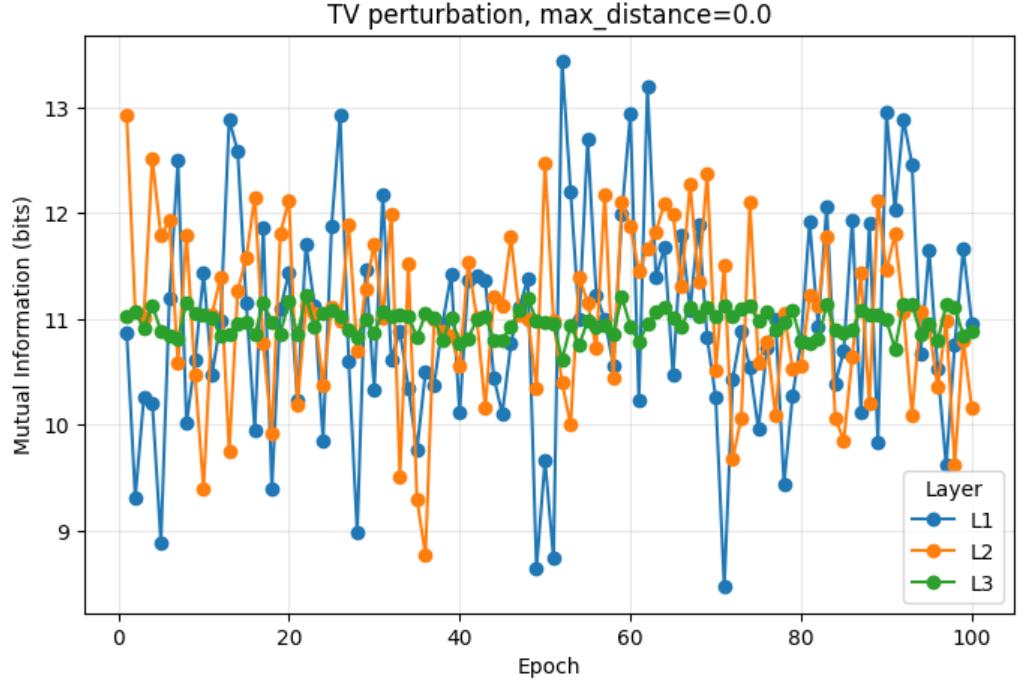
\includegraphics[width=8cm,height=4cm]{ITSL/TV0.png}\hfill
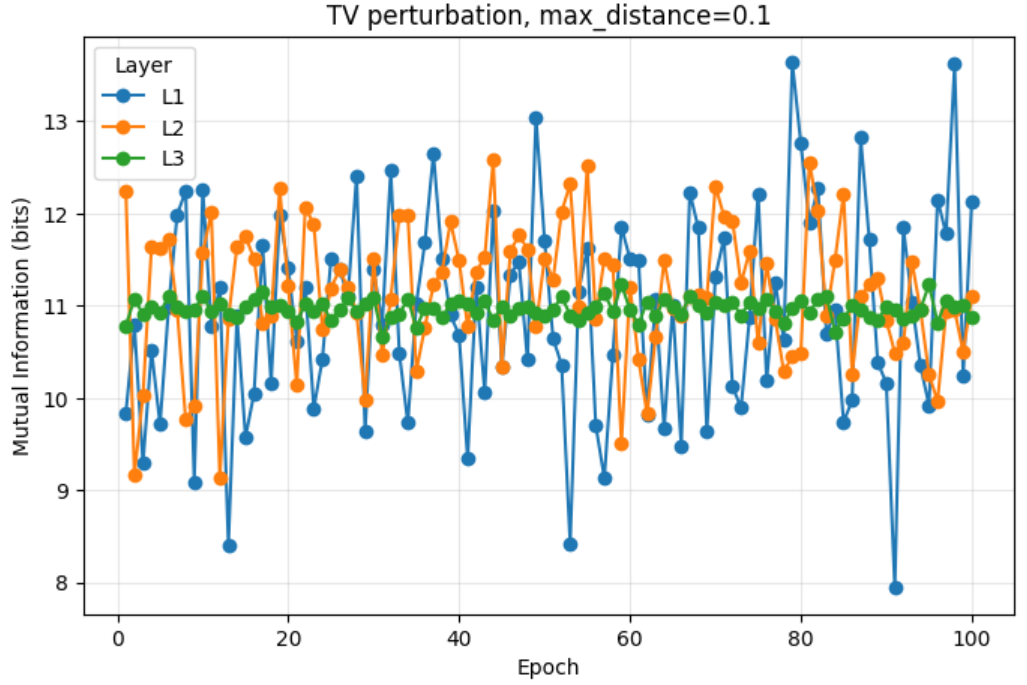
\includegraphics[width=8cm,height=4cm]{ITSL/TV1.png}
\vspace{1em}
% Row 2
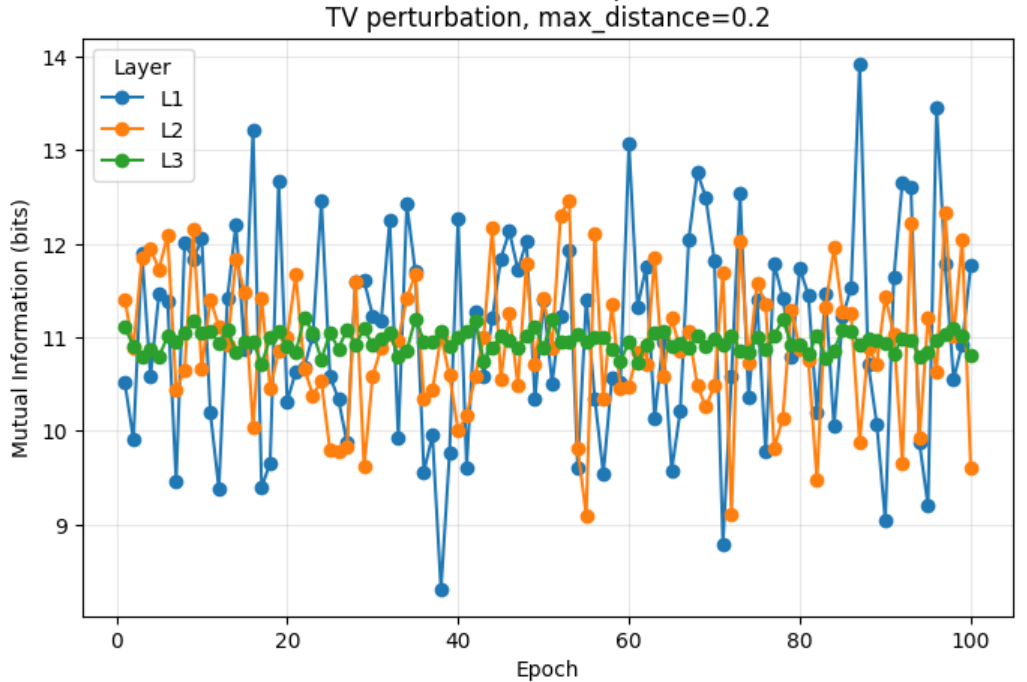
\includegraphics[width=8cm,height=4cm]{ITSL/TV2.png}\hfill
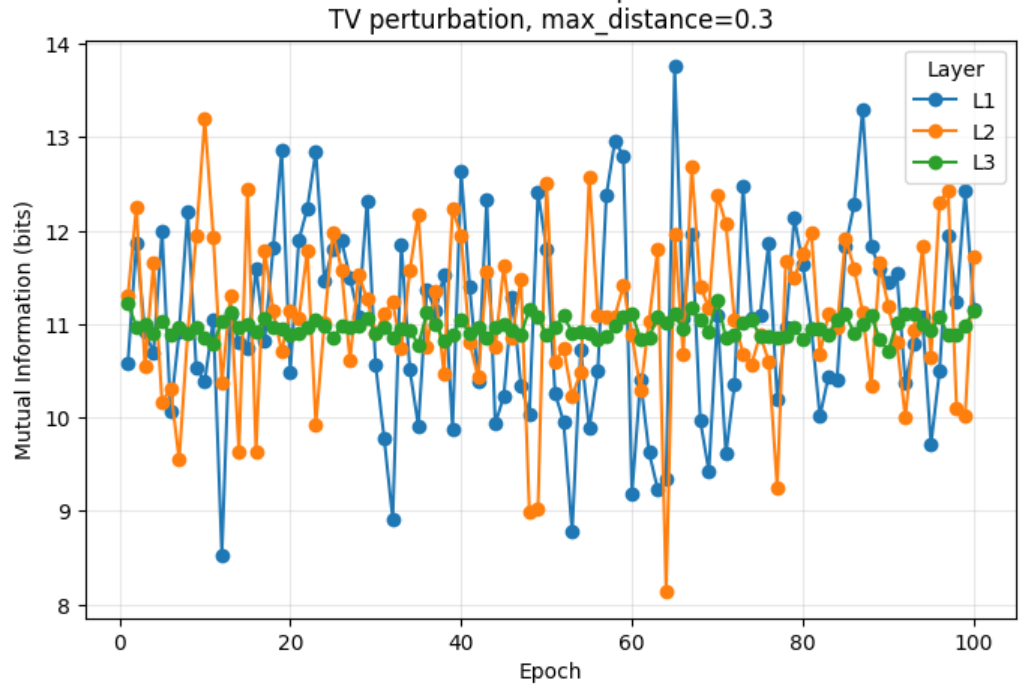
\includegraphics[width=8cm,height=4cm]{ITSL/TV3.png}
\vspace{1em}
% Row 3
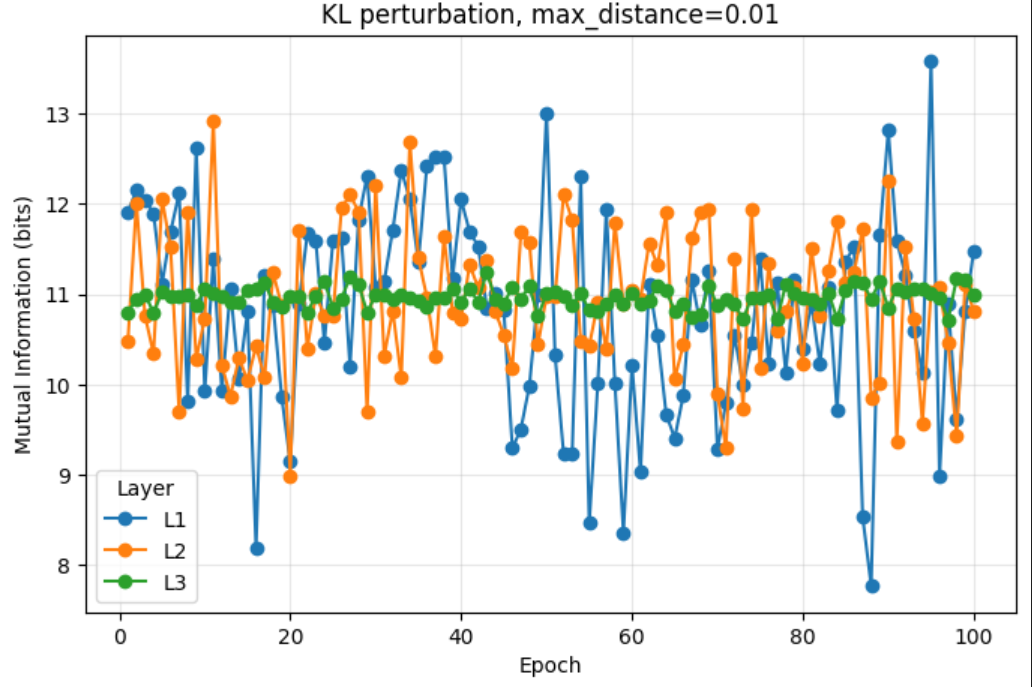
\includegraphics[width=8cm,height=4cm]{ITSL/KL1.png}\hfill
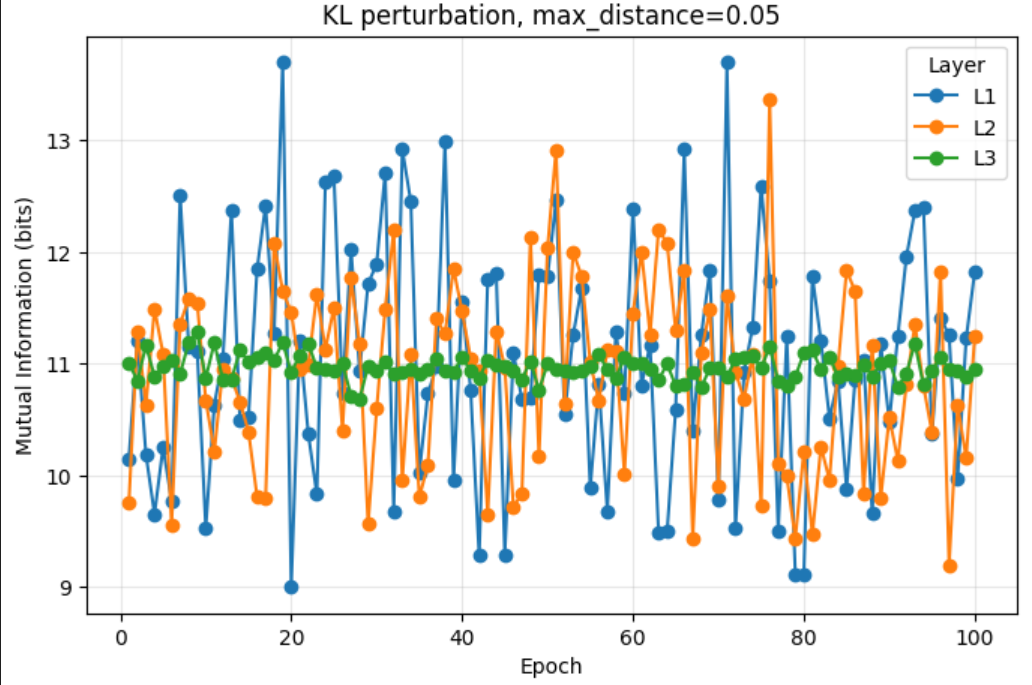
\includegraphics[width=8cm,height=4cm]{ITSL/KL2.png}
\vspace{1em}
% Row 4
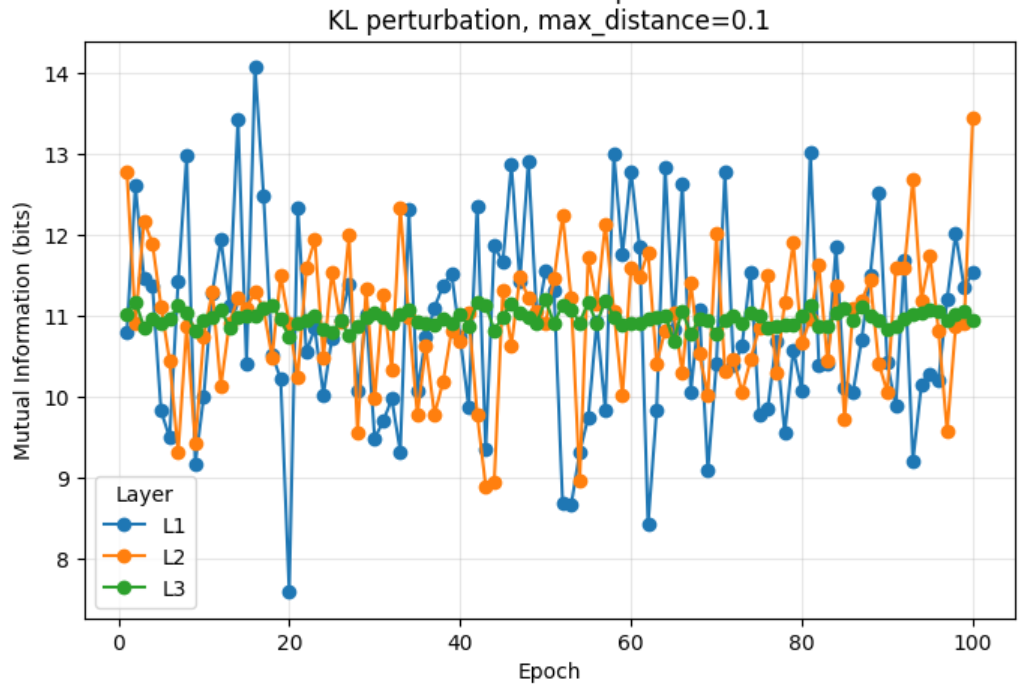
\includegraphics[width=8cm,height=4cm]{ITSL/KL3.png}\hfill
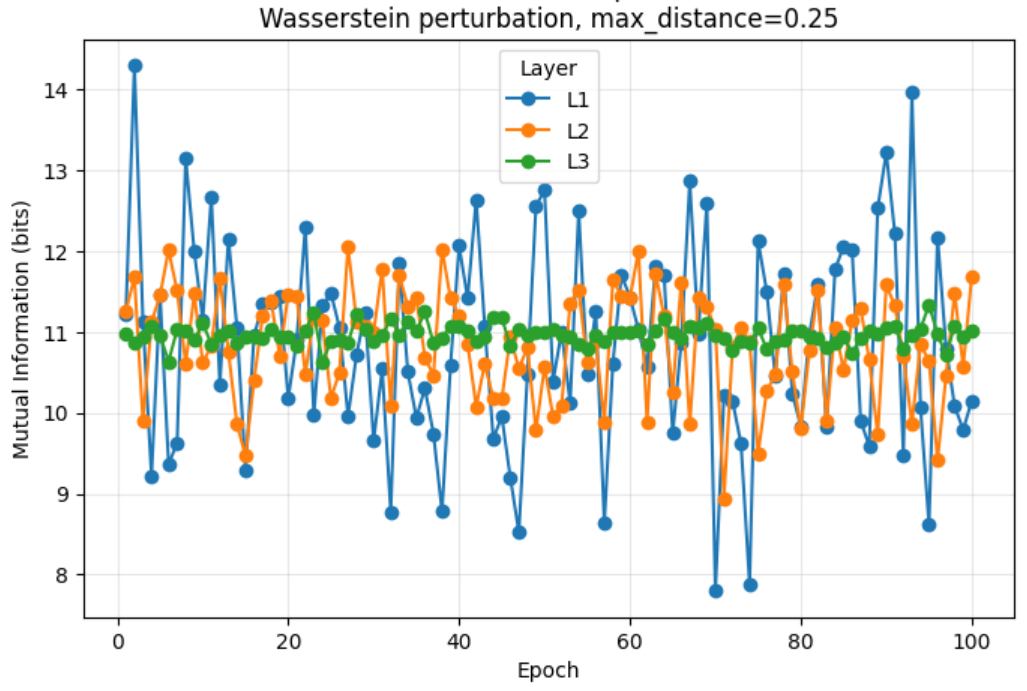
\includegraphics[width=8cm,height=4cm]{ITSL/WS1.png}
\vspace{1em}
% Row 5
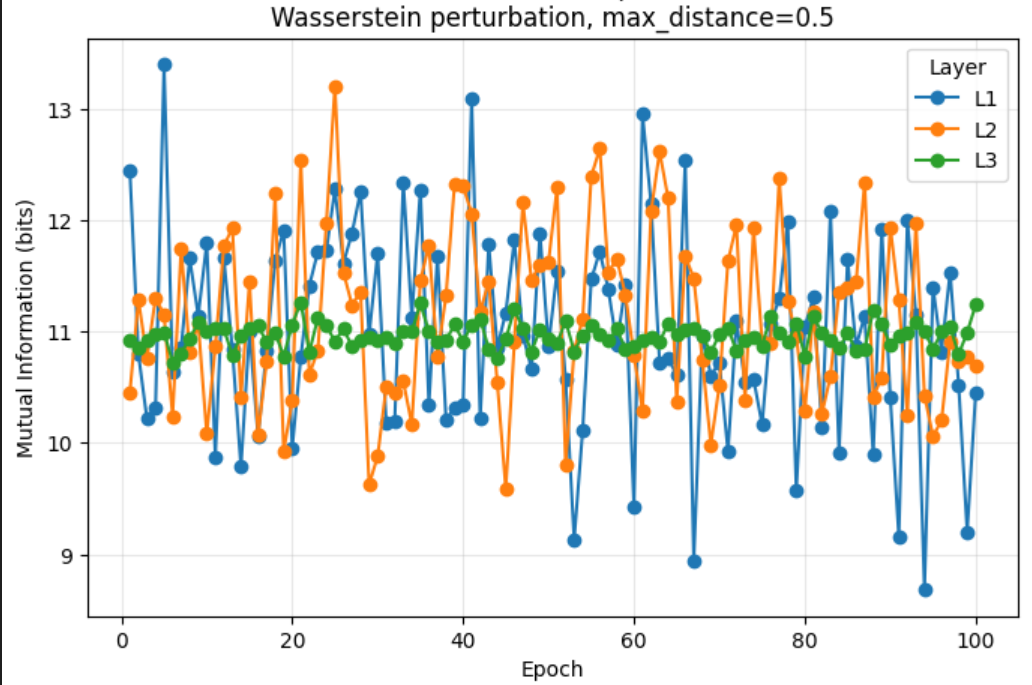
\includegraphics[width=8cm,height=4cm]{ITSL/WS2.png}\hfill
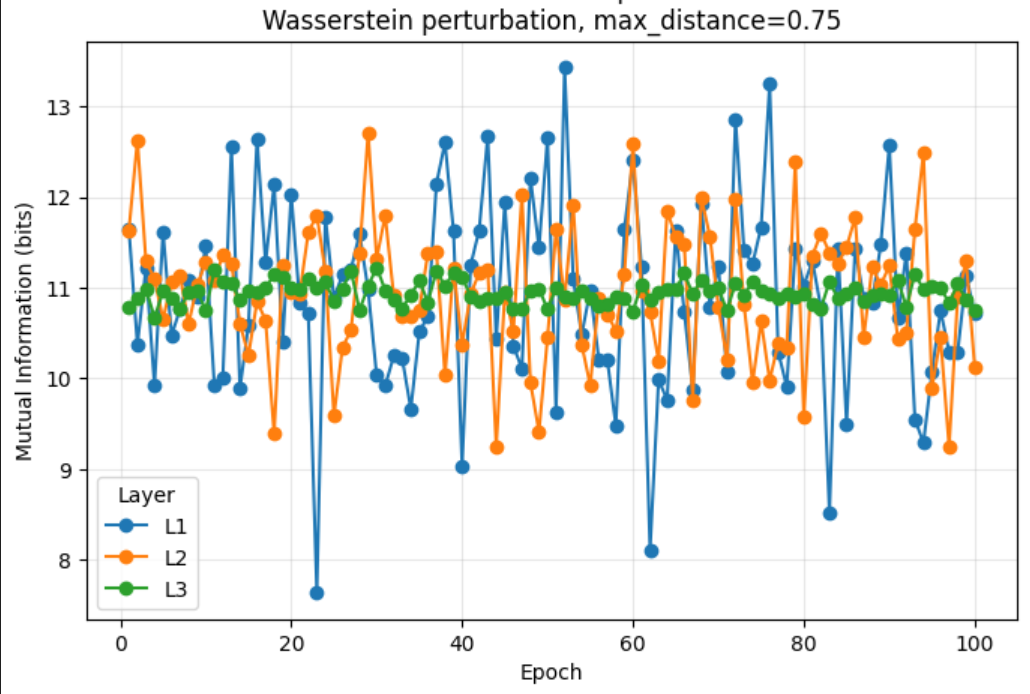
\includegraphics[width=8cm,height=4cm]{ITSL/WS3.png}
\caption{Mutual Information under Distributional Shift. Each of the 10 panels plots $I(X; T_l)$ vs. the magnitude of perturbation for different layers and experimental settings. These plots demonstrate the empirical stability (or lack thereof) of the learned information pathways across various conditions.}
\label{fig:main_results}
\end{figure*}
%====================================================================

\section{Experimental Validation}

\subsection{Experimental Setup}
To validate our theoretical findings, we performed experiments using two models: the fully connected network from \cite{shwartz2017opening} (the SZT model) and a convolutional network for MNIST classification, as described in \cite{goldfeld2019estimating}. We trained these models and, at various epochs, measured the mutual information using the SP estimator. To simulate distributional shifts, we perturbed the test set using methods designed to control the TV, KL, and Wasserstein distances from the original data distribution. For each perturbed dataset, we calculated the mutual information and compared it against the information on the clean dataset.

\subsection{Results}
Figure \ref{fig:main_results} contains our main experimental results. The plots show that mutual information estimates are relatively stable for small perturbations but can vary significantly as the distributional shift increases. The behavior also differs across layers, with deeper layers sometimes exhibiting more sensitivity to shifts, which aligns with the notion that they learn more complex and potentially brittle features.

\section{Future Work}
Our analysis opens several avenues for future research.

First, our theoretical work provided bounds for TV and KL perturbations. A natural next step is to derive a similar bound for the Wasserstein distance. Since Wasserstein distance captures the underlying geometry of the space, a Wasserstein-based bound could provide tighter and more meaningful guarantees, especially for high-dimensional data.

Second, our work focused on analyzing the effects of distributional shifts on models trained with standard Empirical Risk Minimization (ERM). An exciting direction would be to use a Distributionally Robust Optimization (DRO) framework during training. Algorithms like those described in \cite{duchi2018certifying} aim to train models that are explicitly robust to a class of distributional perturbations. It would be valuable to investigate whether models trained with DRO exhibit more stable information planes. This could lead to a new regularization technique aimed at not just improving generalization but also ensuring the stability of the learned information pathways.

\section*{Acknowledgment}
We would like to express our sincere gratitude to our instructor, Dr. Yassaee, for his guidance and support throughout this project. We also thank our project mentor, Mr. Hadavi, for his invaluable feedback and insights. Finally, we acknowledge the foundational work of Ziv Goldfeld, Yury Polyanskiy, and their co-authors, which inspired and enabled this project.


\bibliographystyle{IEEEtran}   % the IEEE BibTeX style
\bibliography{references}

% Command to start appendix on a new page
% \clearpage

% ====================================================================
% ====> APPENDIX SECTION
% ====================================================================
\clearpage

\appendices
\section{Proof of Theoretical Bounds}

We first prove a lemma which bounds the change in mutual information due to a shift in the input distribution.
\begin{lemma}[Continuity of Mutual Information]
Let $\mathcal{X}$, $\mathcal{T}$ be finite alphabets with $|\mathcal{T}|=N_l$. Fix a channel $W(t\mid x)$. Let $P_X, P'_{X}$ be two input distributions such that $TV(P_X,P'_{X}) \le \epsilon$. Let $P_T, P'_{T}$ be the corresponding output distributions. Then
\begin{equation*}
\big| I(X;T)-I(X';T)\big| \le 2\epsilon \log N_l + H_b(\epsilon)
\end{equation*}
where $H_b(\cdot)$ is the binary entropy function. 
\end{lemma}
\begin{IEEEproof}
We follow four steps. Let $I=I(X;T)$ and $I'=I(X';T)$.

\textbf{Step 1: TV contraction under channels.}
The total variation distance between the output distributions is
\begin{align}
    2 \cdot TV(P_T, P_{T'}) &= \sum_t |P_T(t)-P'_{T}(t)| \nonumber \\
    &= \sum_t \left|\sum_x (P_X(x)-P'_{X}(x))W(t\mid x)\right| \nonumber \\
    &\le \sum_t \sum_x |P_X(x)-P'_{X}(x)| W(t\mid x) \nonumber \\
    &= \sum_x |P_X(x)-P'_{X}(x)| \sum_t W(t\mid x) \nonumber \\
    &= \sum_x |P_X(x)-P'_{X}(x)| = 2 \cdot TV(P_X, P_{X'}).
\end{align}
Thus, $TV(P_T,P'_{T})\le TV(P_X,P'_{X})\le\epsilon$.

\textbf{Step 2: Continuity of entropy.}
We first prove an entropy bound.
\begin{lemma}
Let $(U,V)$ be any joint distribution on $\mathcal{T}\times\mathcal{T}$ with $\Pr(U\neq V)=\delta$. Then $H(U\mid V) \le H_b(\delta) + \delta\log(N_l-1)$.
\end{lemma}
\begin{IEEEproof}
Define the indicator $E:=\mathbf{1}\{U\neq V\}$. By the chain rule, $H(U\mid V) = H(E\mid V) + H(U\mid V,E)$. Since $E$ is a function of $(U,V)$, $H(E|U,V)=0$. Thus, $H(U|V) \le H(E) + H(U|V,E)$. Since conditioning cannot increase entropy, $H(E\mid V)\le H(E)=H_b(\delta)$.
Next, $H(U\mid V,E) = (1-\delta)H(U\mid V,E=0) + \delta H(U\mid V,E=1)$.
If $E=0$, then $U=V$, so $H(U\mid V,E=0)=0$. If $E=1$, the support of $U$ given $V=v$ has at most $N_l-1$ values, so $H(U\mid V,E=1)\le \log(N_l-1)$.
Combining these gives the result.
\end{IEEEproof}
Now, let $p,q$ be distributions on $\mathcal{T}$ with $TV(p,q)=\delta$. We can construct a maximal coupling $(U,V)$ with marginals $p,q$ and $\Pr(U\neq V)=\delta$. Then
\begin{equation}
|H(p)-H(q)| = |H(U)-H(V)| \le \max\{H(U\mid V),H(V\mid U)\}.
\end{equation}
Applying the lemma to both terms yields
\begin{equation}
|H(p)-H(q)| \le H_b(\delta) + \delta\log(N_l-1).
\end{equation}
Using this result on our marginals $P_T, P_{T'}$ with $\delta \le \epsilon$:
\begin{equation}
|H(T)-H(T')| \le \epsilon \log(N_l-1) + H_b(\epsilon). \label{eq:marg_bound_final}
\end{equation}

\textbf{Step 3: Change in conditional entropy.}
Let $h(x)=H(W(\cdot\mid x))$. Note $0\le h(x)\le \log N_l$.
\begin{align}
    |H&(T|X) - H(T'|X')| = \left|\sum_x (P_X(x) - P'_{X}(x))h(x)\right| \nonumber \\
    &\le \sum_x |P_X(x) - P'_{X}(x)| |h(x)| \nonumber \\
    &\le \left( \sum_x |P_X(x) - P'_{X}(x)| \right) \max_x h(x) \nonumber \\
    &= 2 \cdot TV(P_X, P'_{X}) \cdot \log N_l \le 2\epsilon \log N_l.
\end{align}

\textbf{Step 4: Combine bounds.}
Using $I=H(T)-H(T|X)$ and the triangle inequality,
\begin{align}
|I-I'| &\le |H(T)-H(T')| + |H(T|X)-H(T'|X')| \\
&\le (\epsilon\log(N_l-1) + H_b(\epsilon)) + 2\epsilon\log N_l \\
&\le 3\epsilon\log N_l + H_b(\epsilon).
\end{align}
This proves the lemma.
\end{IEEEproof}

\subsection{Proof of Theorem 1 (TV Shift Bound)}
We bound the error $\mathbb{E}|I(X'; T_l) - \hat{I}_{SP}|$ using the triangle inequality:
\begin{equation}
\begin{split}
    \mathbb{E}|I(X'; T_l) &- \hat{I}_{SP}| \le \mathbb{E}|I(X'; T_l) - I(X; T_l)| \\
    & + \mathbb{E}|I(X; T_l) - \hat{I}_{SP}|
\end{split}
\end{equation}
The first term is the "Shift Error," bounded by Lemma 1. Using the discretization hypothesis $N_l = K^{d_l}$:
\begin{equation}
\begin{split}
    |I(X'; T_l) - I(X; T_l)| &\le 3\epsilon \log(K^{d_l}) + H_b(\epsilon) \\
    &= 3\epsilon \cdot d_l \log K + H_b(\epsilon)
\end{split}
\end{equation}
The second term is the "Estimation Error" from Goldfeld et al. \cite{goldfeld2019estimating}, given in Eq. (\ref{eq:goldfeld_bound}). Combining the two yields the final result.

\subsection{Proof of Theorem 2 (KL Shift Bound)}
The proof follows from Theorem 1 and Pinsker's inequality, which states $TV(P, Q) \le \sqrt{\frac{1}{2} D_{KL}(P || Q)}$. Given $D_{KL}(P_{X'} || P_X) \le \epsilon$, we have:
\begin{equation}
TV(P_X, P_{X'}) \le \sqrt{\frac{\epsilon}{2}}
\end{equation}
We substitute this new TV bound, let's call it $\epsilon' = \sqrt{\epsilon/2}$, into the "Shift Error" term from Lemma 1:
\begin{equation}
\text{Shift Error} \le 2\epsilon' \cdot d_l \log K + H_b(\epsilon')
\end{equation}
This gives the desired result.





\end{document}